\textit{This chapter will give the reader background information about UAVs and point out a problem SDU is currently facing in two ongoing projects. Further more it will describe the focus of this project and how others have managed to solve it.}
\subsection*{Background}
UAS is an emerging technology used in lots of different areas\cite{gupta2013review}.

Especially quadroters also refereed to as multiroters have started to gain a lot of attention. This is, among other reasons, because it has become cheaper to produce the hardware needed to build a quadroters. Microcontrollers have become powerful enough in order to make it possible to implement control and navigation algorithms on a quadroters.\cite{gibiansky2010quadcopter}

A multiroter works by having three or more rotors mounted with equal distance from the centrum of the multiroter.
Not all roters of the multiroter spins the same way in order to compensate for the torque generated by the multiroter.
A multiroter is usually equipped with a flight controller, battery, three or more electronic speed controllers and rotors.
The multirotor balances using its flight controller that controls the velocity and thereby the thrust of each rotor. Usually a rotor is brushless which means it has three phases that needs to be turned on and off, so called commutation, at the right time. The job of the Electric Speed Controller is to do the commutation depending on the speed sent from the flight controller. \\

One of the challenge concerning multirotors is the amount of energy they are capable of carrying. If the drone is equipped with a heavy camera or other kind of payload, then the flight time begins to decrease. 
By looking at the nature, one can see how small animals like ants and birds manage to cooperate and thereby build or move bigger things that they would not be able to do on their own. This way of small independent, decentralized units working together is called a swarm\footnote{\url{https://en.wikipedia.org/wiki/Swarm\_intelligence}}.\\
By making multirotors smaller, they get more efficient, their flight time increase and they get cheaper but of the cost of their ability to lift\cite{1_kumar_2016}. Therefore an idea would be to make small multirotors cooperate to solve more heavy and complex tasks. \\

Multirotors can be used in a wide range of applications.
If the multirotor is equipped with a camera it can quickly provide an overview of a fence, wiring, lamps etc. Multiroters is usually used in applications outside which among other reasons, might be caused by the requirement of GPS signal being available.
Most multicopters are capable of flying indoor however they often has little knowledge about where they are since they lack GPS indoor. It limits the applications multirotors can be used for indoor. 
A research project named UAWORLD has just started which will focus on doing indoor flying.\footnote{\url{http://innovationsfonden.dk/da/case/droner-rykker-indendoers-med-dansk-teknologi-0}}. They will focus on making multirotors robust and safe enough in order to let multirotors fly indoor. They are going to develop the system in cooperation with GamesOnTrack.com which delivers the indoor 3D localization system. GamesOnTrack's localization system uses beacons and triangulation to localize objects.\footnote{More information is not available online} The are sure that drones will be used indoor at hotels, hospitals, schools and offices. 

The GPS available outdoor has an accuracy of 3.5 meter \footnote{http://www.gps.gov/systems/gps/performance/accuracy/} which might be adequate depending on the applications. In most flight controllers, the GPS is fused with onboard sensors like accelerometer and gyroscope however the positioning is still not adequate if the multirotor is supposed to fly close to an object within centimeters. 

Even though GPS is usually available outdoor there might be places where no GPS signal is available eg. In forests or cities with high buildings. 
In indoor as well as outdoor applications where absolute positioning is required but GPS is not available alternative solutions such as radio triangulation, vision or totalstations could be used. 
However most of the multiroters available on the marked only supports using their build-in GPS which might be a limitation if GPS is not available but accurate flying is necessary.


At the time of writing, SDU is collaborating with HCA airport to find anomalies in fences.\\ 
\textit{Airports are burdened by a number of required inspection tasks to maintain a high level of safety and security.
Some of these tasks may advantageously be performed by a drone rather than manually, as is is currently, and save time and resources.
In this project they are targeting a specific need for frequent inspection of the fence surrounding the airport shown in figure \ref{fig:hca_fence}. 
The inspection concerns fence holes or similar anomalies. We hypothesize that a drone is 
capable of unsupervised autonomous inspecting the airport fence detecting small holes down 
to a radius of 5 cm.} \footnote{Application sent to Energi Fyns Udviklingsfond which has been granted, Ansøgning 2015-01-30 Energi Fyns Udviklingsfond-1.pdf on USB}

\begin{figure}[H]
    \centering
    %(or a blank line to force the subfigure onto a new line)
    \begin{subfigure}[b]{0.45\textwidth}
        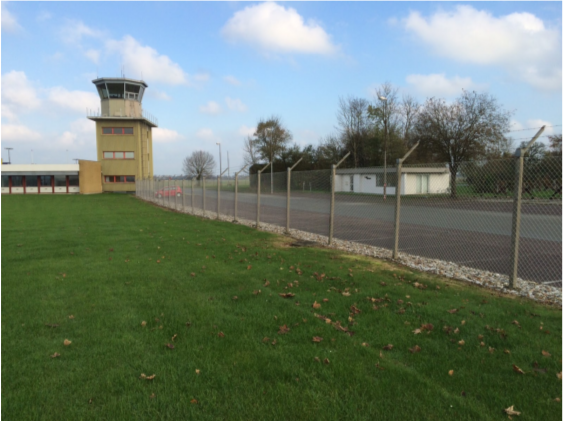
\includegraphics[width=\textwidth]{graphics/hca_fence.png}
        \caption{Part of the fence surrounding HCA Airport.}
        \label{fig:hca_fence}
    \end{subfigure}
        ~  %add desired spacing between images, e. g. ~, \quad, \qquad, \hfill etc. 
    %(or a blank line to force the subfigure onto a new line)
    \begin{subfigure}[b]{0.45\textwidth}
        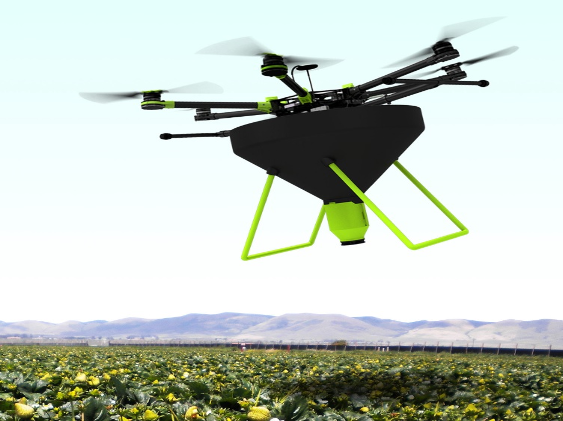
\includegraphics[width=\textwidth]{graphics/organicdrone.png}
        \caption{Drone spreading ladybirds and gall midges to avoid spreading pesticides in organic crops}
        \label{fig:organicdrone}
    \end{subfigure}
   \label{fig:sdu_projects}
\end{figure}

In order to avoid flying into the fence and to fly accurate enough for the camera to film, it is required to have an vertical accuracy of 2-3 cm \footnote{Henrik Egemose Schmidt - Drone inspection of fences}

In another project, SDU is working together with Ecobotix ApS, Aarhus Univercity and EWH BioProduction ApS, to avoid the need of pesticides in organic crops. Pesticides are  chemical substances used to kill pests from the crops. When using pesticides a health risks exists for those who eat the crops. The use of pesticides also reduce the amount of diversity in nature since it is also killing beneficial organisms and potentially harm other animals in the food chain like birds. If nothing is used the crops might die, and that is very expensive to the farmer. The project has been granted 8.356.126 kr. from GUDP \footnote{\url{http://naturerhverv.dk/tvaergaaende/gudp/gudp-projekter/2015/oekodrone-skal-sprede-mariehoens-i-stedet-for-pesticider/} last visited 18-04-2016}\\
They intend to use multirotors to spread bugs like ladybirds and gall midges, over the crops to eat pests as shown in fugure \ref{fig:organicdrone}. \\
It is required the drones fly approximately 1 meter above ground at 1.5 meter/sec. It is therefore necessary to use an RTK-GPS in order to avoid hitting the ground in case of bumps in the fields. \footnote{Jensen, K.; Larsen, R.; Laursen M.S.; Neerup, M.M.; Skriver, M. and Jørgensen, R.N. Towards UAV contour flight over agricultural fields using RTK-GNSS and a Digital Height Model. Accepted for oral presentation at CIGR-AgEng June 2016.}\\


Many different flight controllers exists on the marked. SDU UAS has decided to use AutoQuad since, among other reasons, the code is Open Source \footnote{Quatos, which is their control algorithm is not Open Source.} and the multiroters show reliable and steady flying. An AutoQuad multiroter delivered by ViaCopter\footnote{\url{https://viacopter.eu/}} usually comes with with the AutoQuad flight controller M4, Electronic Speed Controllers( ESC32 ) and rotors. One of ViaCopters smallest drones is delivered without Electronic Speed Controllers since H-bridges used to control the velocity of the motors are build into the M4 flight controller.
ViaCopter can deliver drones in different sizes but their flight controller is the same. This means that code developed for ViaCopters Ladybird can be deployed on a large drone and it will continue to work\footnote{Assumed the developer did not break important lowlevel tasks}. However AutoQuad does not support any other source of absolute positioning other than using its onboard GPS. \\

Because of the research-projects at SDU, there is a need for being able 


\begin{figure}[H]
    \centering
    \begin{subfigure}[b]{0.3\textwidth}
        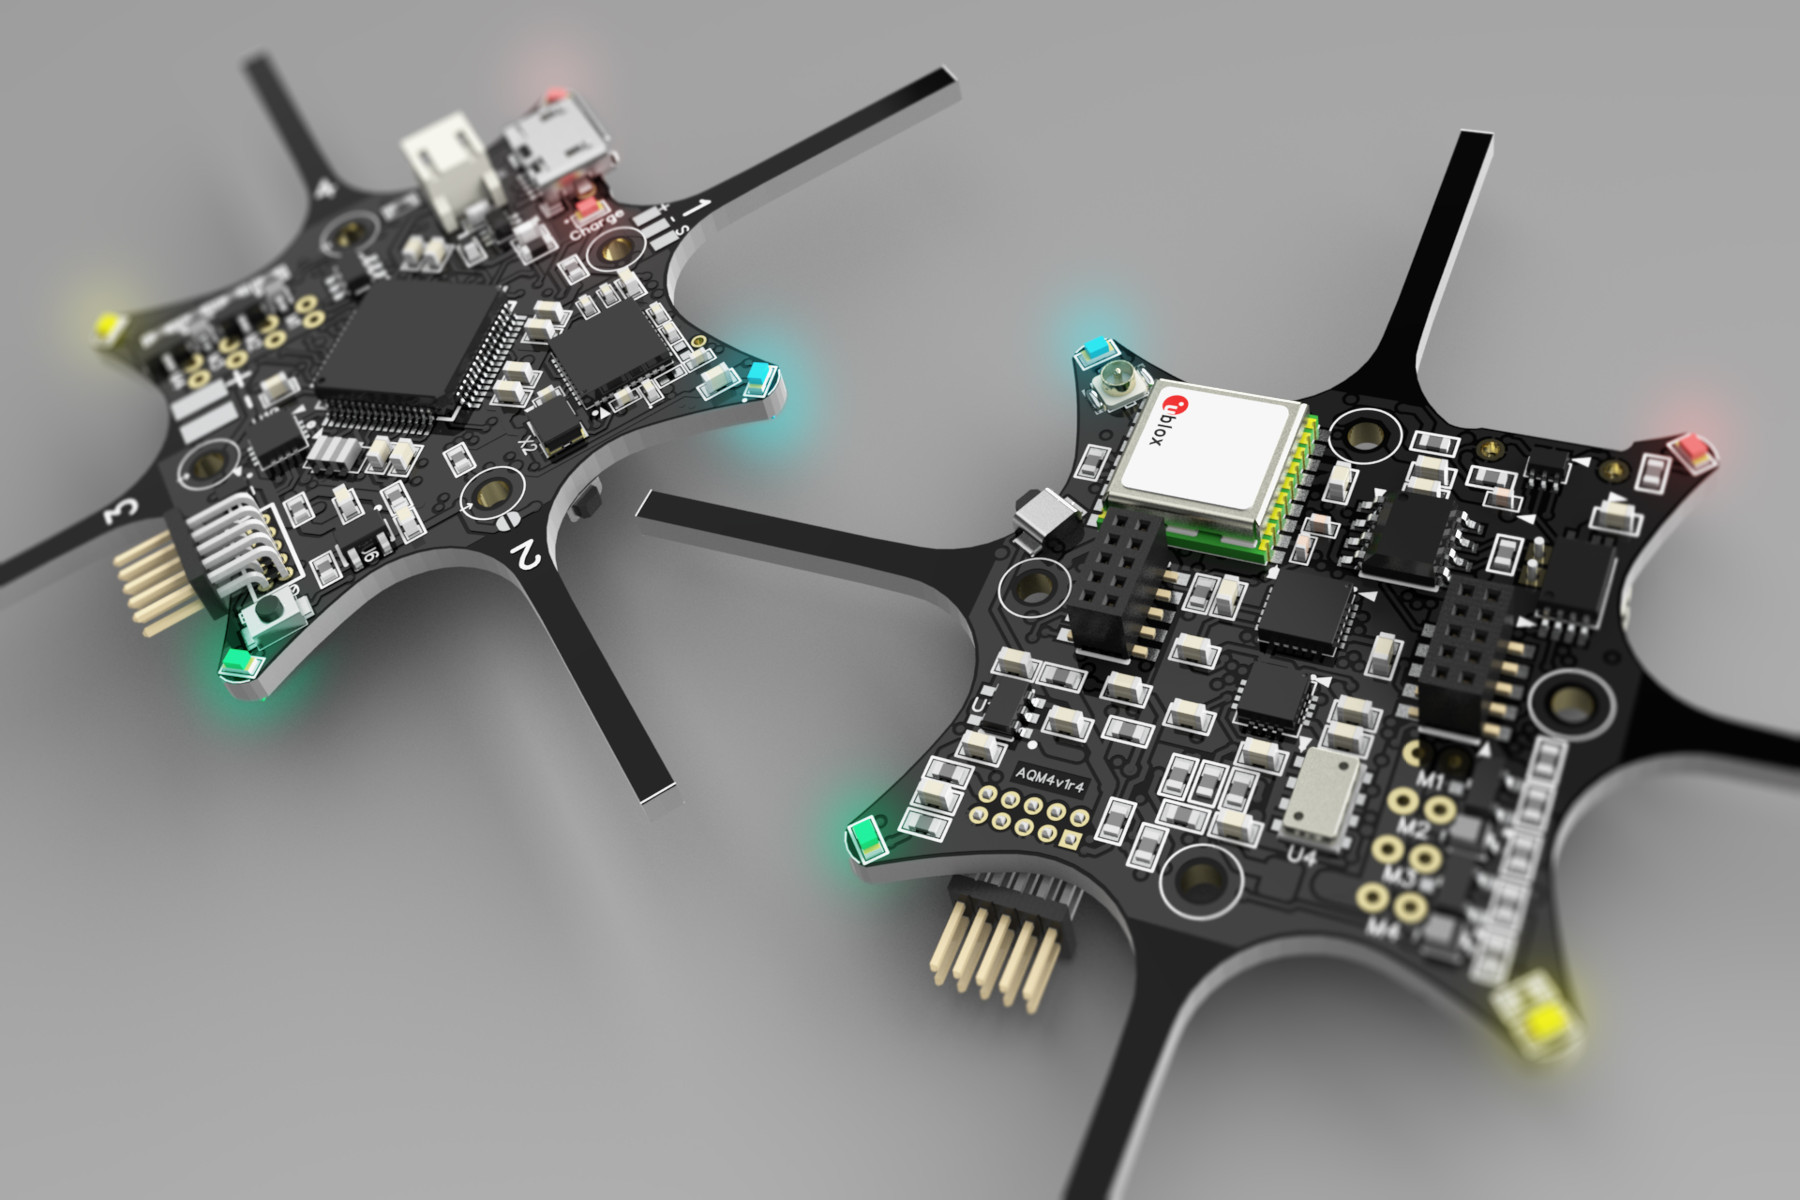
\includegraphics[width=\textwidth]{graphics/M4_demo}
        \caption{M4 flight pilot}
        \label{fig:gull}
    \end{subfigure}
    ~ %add desired spacing between images, e. g. ~, \quad, \qquad, \hfill etc. 
      %(or a blank line to force the subfigure onto a new line)
    \begin{subfigure}[b]{0.3\textwidth}
        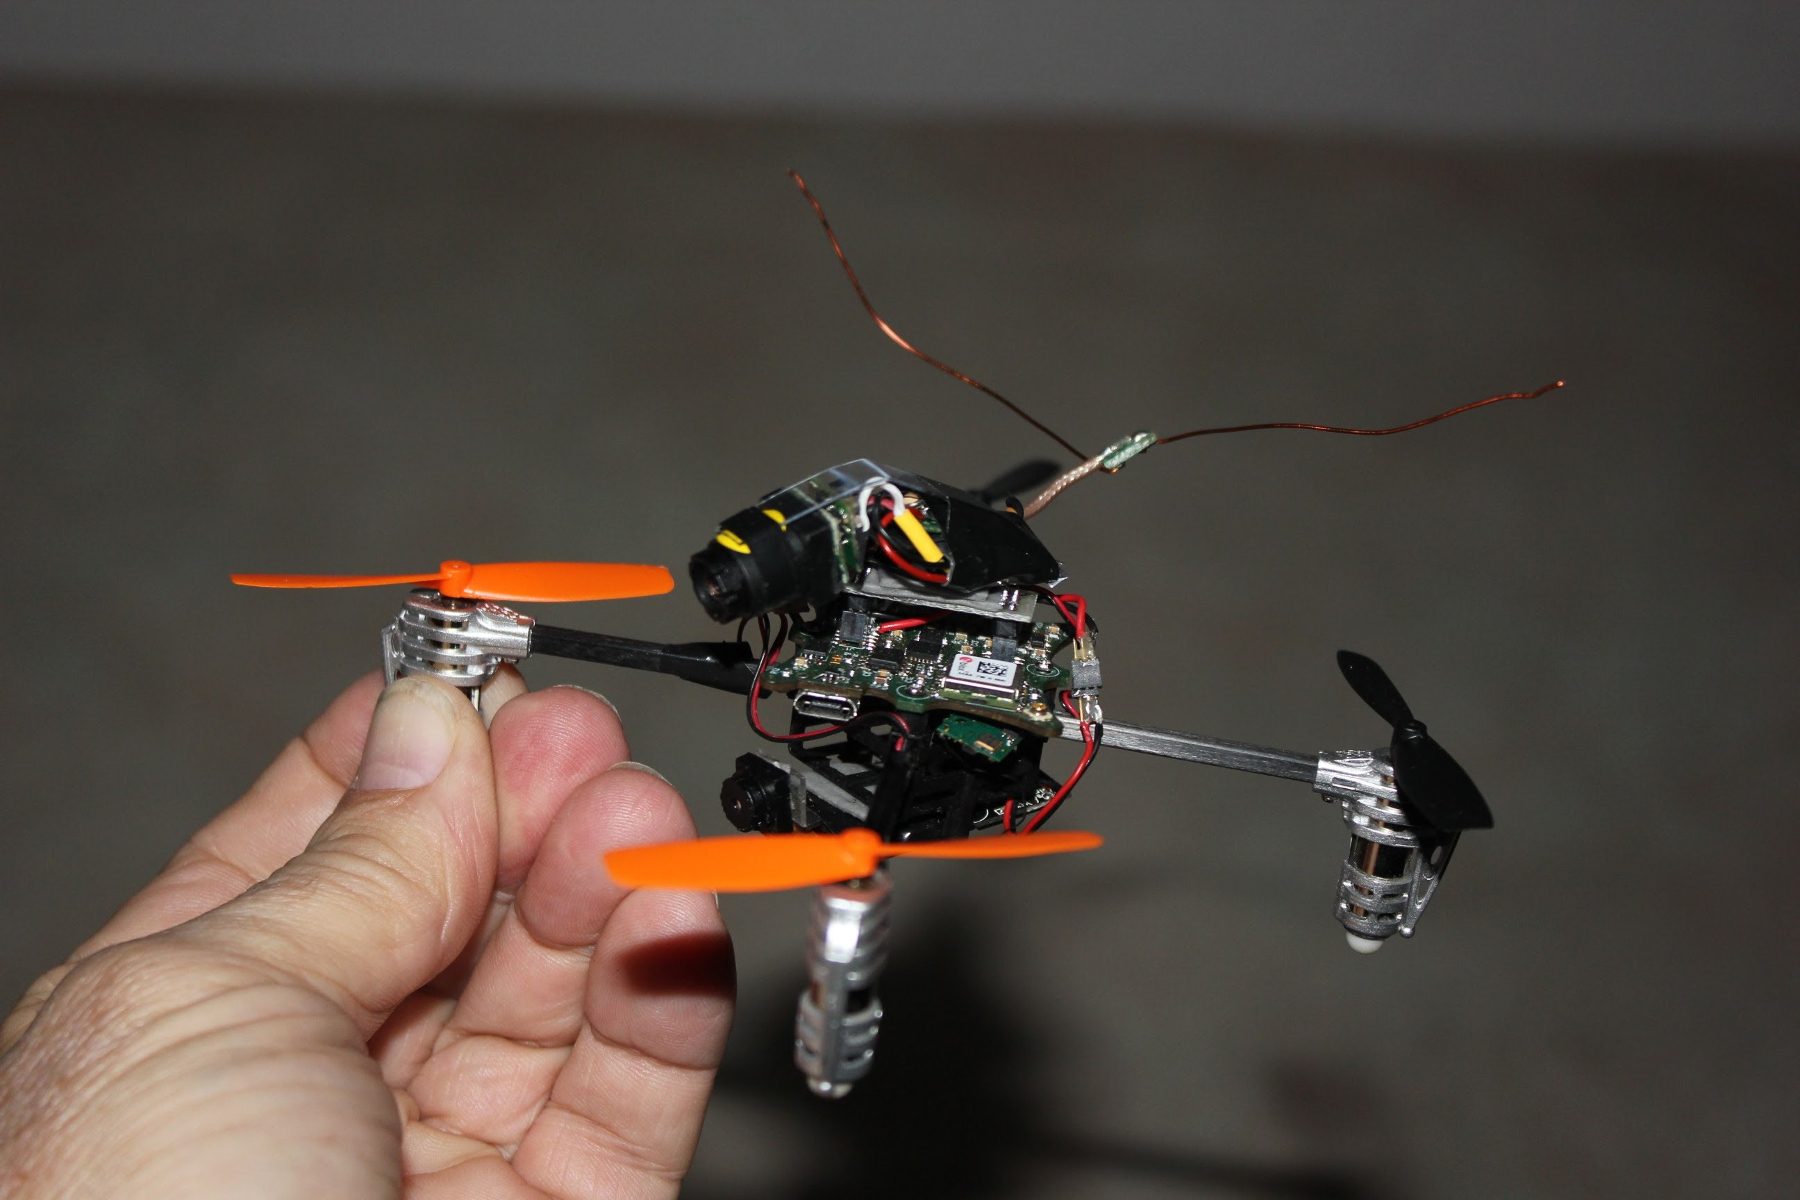
\includegraphics[width=\textwidth]{graphics/ladybird}
        \caption{Ladybird with mounted M4}
        \label{fig:tiger}
    \end{subfigure}
    ~ %add desired spacing between images, e. g. ~, \quad, \qquad, \hfill etc. 
    %(or a blank line to force the subfigure onto a new line)
    \begin{subfigure}[b]{0.3\textwidth}
        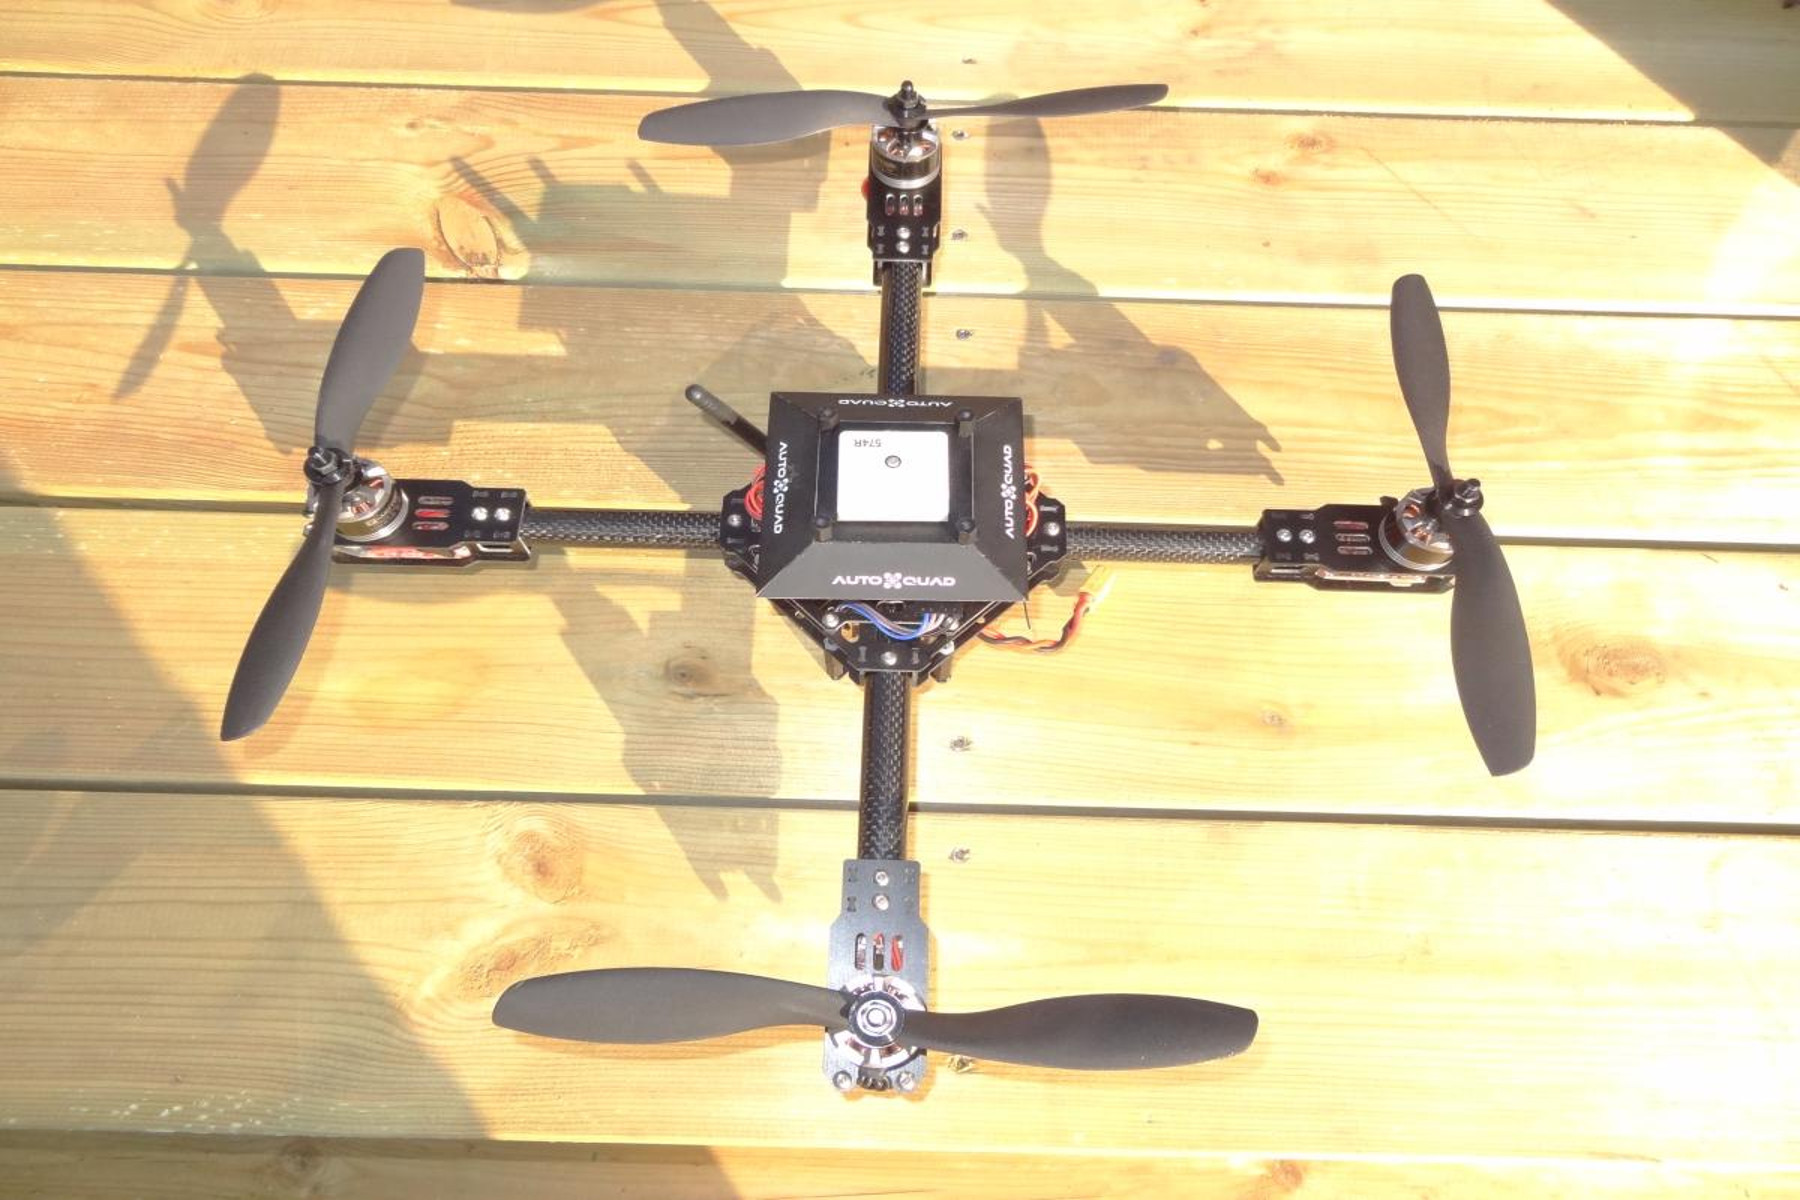
\includegraphics[width=\textwidth]{graphics/eduquad.jpg}
        \caption{Eduquad with M4 + ESC32}
        \label{fig:mouse}
    \end{subfigure}
    \caption{Pictures of AutoQuad hardware}\label{fig:AQ_hw}
\end{figure} 



\newpage
\section{Problem Statement}
The current AutoQuad version does not support any other source of global positioning than the onboard GPS and thereby does not support accurate flying better than GPS and if GPS is not available, there i is no alternatives supported. For AutoQuad to be used in applications requiring high accuracy or where GPS is unavailable this functionality is needed. \\


\section{Related Work}
In order to find relevant research about drones flying indoor, a few search phrases was conducted.
The following keywords were used to create different phases: Indoor, environment, swarm, localization, AutoQuad, quadrotor, mini UAV, test facilities, ETH, accurate, RTK, totalstation.
Based on the keywords a few papers was deemed relevant to the project and has been combined in order to give the reader an overview within the field of this project. \\

Developers of AutoQuad did previously try to implement RTKLib \footnote{http://www.rtklib.com} in AQ. Unfortunately they did manage to make it work as expected \footnote{Jussi Hermansen, owner of \url{http://ViaCopter.eu}}.\\

One of the big players within the field of indoor navigation and controlling multiple drones accurately is the university ETHzûrich and their Institute for Dynamic Systems and Modelling \footnote{\url{http://www.idsc.ethz.ch/research-dandrea/research-projects/aerial-construction.html}}. They have developed a test flying area they call "Flying Machine area" which provides facilities for doing prototype testing of new control algorithms \cite{lupashin2014platform}. The FMAs dimensions is 10*10*10m and provides nets to protect people and mattresses to protect the drone  if a crash. The FMA has further been developed into a mobile installation to be used in demonstrations in Europe and North America. One of their demonstrations where used in a TED video about multiroters and their capabilities \footnote{https://www.ted.com/talks/raffaello\_d\_andrea\_the\_astounding\_athletic\_power\_of\_quadcopters}.
The multiroter usually used in the FMA is Ascending Technologies' Hummingbird with custom wireless communication and electronics. \\
They have build it as a module design in order to be easy to replace parts of their system by simulations and to make it scalable.
One of their modules is a copilot that implements an accident handler in case of user-code crashing or sending invalid commands to the drones.
They are using UDP multicast packets as communication between ground computation and flying objects. The use of UDP multicast packets between modules since to makes the system more simple but also to avoid the need of buffers to handle unsuccessful transmissions and retransmissions. \\
In order to detect the quadroters they are using a commercial motion capture system. Three reflective markers is mounted on each flying object in order to obtain attitude and position. They are using three cameras to reduce the risk of false positive even though two cameras would be enough to get a flying objects 6D position.\\
 
 
\cite{kang2015indoor} proposes a more simplistic approaches to do indoor navigation.
They use bluetooth 4 to communicate between their multiroter(Rolling Spider) and an android phone which controls the multiroter.
They have mounted a camera on the ceiling to detect the target and the flying multiroter.
By doing background subtraction they can detect where the drone is in the frame by subtracting the background from each frame \cite{wikiBackgroundsubtraction}. 
By doing a convolution sum, the targets can be located. By analyzing the pixels around the location of the multiroter, they can get the heading. \\

\cite{sanchez2014system} proposes a framework to accelerate the process of prototyping multiroters behaviors. Their framework is designed for a swarm of drones to fly in a environment with obstacles. One of their design requirements is, that the framework should be highly decoupled from the application the researcher is testing in order to speed up the development process. 
Position estimates is obtain by using onboard IMU and optic flow. To avoid expensive motion capture systems they have used markers that can easily be recognized by cameras mounted on the drones to get a absolute 3D estimate. Each obstacle got a ArUco-marker \cite{Aruco2014} that can be detected by the front camera mounted on the multiroter. \\
They have decided to use ROS as middleware to provide generic interfaces between the modules used in their framework. Different multiroters can be used as long they use the same interface. Communication between multiroters and ground station(if used) is done using WIFI. \\


The most common type of indoor localization is using vision where the camera is either mounted in the environment or where the drone is equipped with cameras to obtain position estimates.\\
\cite{stirling2012indoor} uses a different approach where they use a \textit{Robot Sensor Network} to map the environment.
The idea is that each drone can either be a beacon or explorer. Each drone alternates between these two states. Beacons stays still below the ceiling without moving while explorer flies around to unknown locations. Beacons emit IR light in order to triangulate beacons position.  Beacons detecting unexplored locations calls for explorer that will become beacons and so forth until the environment is mapped. To synchronize the beacons 2.4 ghz WIFI is used. When the environment is mapped, graph searching algorithms can be used to find a path through the environment.


\section{Hypothesis}
If each drone's 2D position is obtained using vision and spoofed into the drone using CAN, then it is possible for at least 3 drones to follow a leader drone with a preprogrammed flight path and keep a euclidean distance at 50 cm within plus minus 10 cm to the leader and its neighbours.
\section{Aim of project}
The aim of this project is to test the hypothesis by making an indoor flying environment to make 3 multirotors follow a leader multirotor. Since a need from SDU has arisen of sending RTK GPS coordinates into AutoQuad, this will also be used to test and to contribute to a scientific paper.



